% 12pt 打底，不是模板的 9pt。
% 会议 talk 与组会分享的口径不同：页面高 255.1pt，PowerPoint 16:9 页面高 540pt，
% 换算系数 2.117。社区惯例是正文不小于 24pt（PowerPoint 口径），折回来要 11.3pt。
% 模板的 9pt 打底 + 密集帧套 \small，实测正文落在 7–8pt，等效只有 15–17pt。
% 代价是版面容量降到 (8/12)^2 ≈ 44%，每页内容必须砍掉一半以上——这是目的不是副作用。
\documentclass[aspectratio=169,12pt]{beamer}
% !TEX root = main.tex
% ============================================================
% 共用 preamble —— 随 deck 自带，改这里只影响本 deck
% ============================================================
% moloch 只支持四个选项：progressbar / sectionpage / subsectionpage / background
% （metropolis 的 numbering、block 靠 \patchcmd 实现，moloch 砍掉了，走 beamer 标准模板）
% sectionpage=none：12 分钟的 talk 不出章节页（见 main.tex 的说明）。
% \section{} 照写，frametitle 上的进度条要靠它。
\usetheme[progressbar=frametitle,
          sectionpage=none]{moloch}
\usepackage[UTF8]{ctex}
\usepackage{tikz}
\usepackage{booktabs}
\usepackage{makecell}
\usepackage{amsmath,amssymb}
\usetikzlibrary{calc,positioning,arrows.meta}

% ------------------------------------------------------------
% 版面密度
% beamer 的 pt 是相对 453.54pt 宽的页面算的，PowerPoint 是相对 720pt。
% 同样点数，beamer 里的字视觉上大 1.6 倍——照搬 pptx 的 11pt 必然溢出。
% 这里压紧列表间距；字号在 \documentclass 上用 9pt 打底。
% ------------------------------------------------------------
% 不要用 enumitem：它一加载就接管 enumerate，与 beamer 的 \labelenumi
% 互相引用，编译时无限递归报 TeX capacity exceeded。改用钩子只压间距。
\usepackage{etoolbox}
\AtBeginEnvironment{itemize}{\setlength{\itemsep}{2pt}\setlength{\parskip}{0pt}}
\AtBeginEnvironment{enumerate}{\setlength{\itemsep}{2pt}\setlength{\parskip}{0pt}}

% ------------------------------------------------------------
% 配色（沿用既有 pptx deck 的 design tokens）
% ------------------------------------------------------------
\definecolor{cPrimary}{HTML}{1B3A5C}
\definecolor{cAccent}{HTML}{2E6CA4}
% 深色块（封面 / section 页 / frametitle 背景）单独一个颜色，
% 与正文强调色 cPrimary 解绑——改标题栏配色只动这两行
\definecolor{cHeader}{HTML}{2E6CA4}
\definecolor{cHeaderAccent}{HTML}{8FBFE0}
\definecolor{cAccentLight}{HTML}{E8F0FE}
\definecolor{cAccentPale}{HTML}{F4F8FE}
\definecolor{cText}{HTML}{333333}
\definecolor{cTextLight}{HTML}{666666}
\definecolor{cGreen}{HTML}{2E7D32}
\definecolor{cRed}{HTML}{C62828}

\setbeamercolor{normal text}{fg=cText}
\setbeamercolor{alerted text}{fg=cRed}
\setbeamercolor{example text}{fg=cGreen}
\setbeamercolor{palette primary}{bg=cHeader, fg=white}    % 标题页 / section 页
\setbeamercolor{frametitle}{bg=cHeader, fg=white}
% moloch 的 progress bar 默认从 alerted text 派生（fg 红、bg 暗红），只覆盖 fg
% 会在 section 页留下一条红线。两个场景底色相反，所以分开设：
%   head/foot  画在深色 frametitle 上 → 亮前景
%   section page 画在浅色页面上 → 深前景
\setbeamercolor{progress bar}{fg=cHeaderAccent, bg=cHeader!20!white}
\setbeamercolor{progress bar in head/foot}{fg=white, bg=cHeader!55!white}
\setbeamercolor{progress bar in section page}{fg=cHeader, bg=cHeader!15!white}
\setbeamercolor{title separator}{fg=cHeaderAccent, bg=cHeader}
\setbeamercolor{block title}{bg=cAccentLight, fg=cPrimary}
\setbeamercolor{block body}{bg=cAccentPale, fg=cText}

% 页码用 beamer 标准模板（不是 metropolis 的 frame numbering）
\setbeamertemplate{page number in head/foot}{%
  \insertframenumber{}/\inserttotalframenumber}
\setbeamerfont{page number in head/foot}{size=\tiny}
\setbeamertemplate{blocks}[rounded][shadow=false]

% 三色 block：block=蓝（常规补充）/ exampleblock=绿（结论、好消息）/ alertblock=橙（矛盾、问题）
% 讲稿里"不是现在该念的那块"。比 cTextLight 淡得多——它只要能读出轮廓、
% 供眼睛确认上下文位置即可，真正要读的是 \speechon 那块。
\definecolor{cSpeechOff}{HTML}{E7E6E6}
\definecolor{cGreenBg}{HTML}{E8F5E9}
\definecolor{cWarnBg}{HTML}{FFF3E0}
\setbeamercolor{block title example}{bg=cGreenBg, fg=cGreen}
\setbeamercolor{block body example}{bg=cGreenBg, fg=cText}
\setbeamercolor{block title alerted}{bg=cWarnBg, fg=cRed}
\setbeamercolor{block body alerted}{bg=cWarnBg, fg=cText}

% ------------------------------------------------------------
% 规约代码（第 8、9 帧）。模板不带 listings，这里按 deck 需要加。
% 用 lstlisting 的帧必须写 \begin{frame}[fragile]。
% 字号 \small 在 12pt 类下是 11pt，等效 PowerPoint 23pt——代码比正文小一档
% 是可以的（听众会盯着看），但不能再小。
% ------------------------------------------------------------
\usepackage{listings}
\definecolor{cCodeBg}{HTML}{FAFAFA}
\definecolor{cCodeKw}{HTML}{1B5E8C}
\definecolor{cCodeType}{HTML}{2E7D32}
\lstdefinestyle{spec}{
  basicstyle=\ttfamily\small,
  backgroundcolor=\color{cCodeBg},
  frame=single, rulecolor=\color{black!20},
  framesep=5pt, xleftmargin=4pt, xrightmargin=4pt,
  keywordstyle=[1]\color{cCodeKw}\bfseries,
  keywordstyle=[2]\color{cCodeType},
  keywords=[1]{configuration,topology,protocol,property,nodetype,link,var,thread,route},
  morekeywords=[2]{Client,Switch,Controller,Server},
  commentstyle=\color{cTextLight}\itshape,
  comment=[l]{//},
  showstringspaces=false,
  aboveskip=0pt, belowskip=0pt,
}

% 表格里的对勾/叉（Fandol 没有这些字形，走 pifont）
\usepackage{pifont}
\newcommand{\cmark}{\textcolor{cGreen}{\ding{51}}}
\newcommand{\xmark}{\textcolor{cRed}{\ding{55}}}

% ------------------------------------------------------------
% 封面版式：左半论文信息，右半下方会议信息
% moloch 原版把 title/subtitle/author/institute/date 从上往下堆成一列，
% 16:9 页面下右半边整个空着。这里改成左右分栏，右半用 \vfill 压到底部。
% 论文自身的信息（作者、发表处）走 \paperinfo，与 \author/\institute 分开。
% ------------------------------------------------------------
\newcommand{\insertpaperinfo}{}
\newcommand{\paperinfo}[1]{\renewcommand{\insertpaperinfo}{#1}}

% moloch 给 author 和 date 设了 \small，institute 漏了，掉回 beamer 默认的
% \scriptsize，封面上 NetLab 比上下两行都小一档。补齐到同级。
\setbeamerfont{institute}{size=\small}

% 分隔线：moloch 原版用 \textwidth，在 minipage 里会顶出去，改用 \linewidth
\newcommand{\titlerule}{%
  \tikzexternaldisable%
  \begin{tikzpicture}
    \fill[cHeaderAccent] (0,0) rectangle (\linewidth, 0.4pt);
  \end{tikzpicture}%
  \tikzexternalenable\par%
}

\setbeamertemplate{title page}{%
  \begin{minipage}[t][0.86\textheight][t]{\textwidth}
    \vspace*{0.10\textheight}
    % --- 左半：论文 ---
    % 模板给 0.66（右下要留给 \author/\institute）。这份 deck 右下只有会议信息，
    % 而作者列表五个人一行放不下会折行，所以放宽到 0.82。
    \begin{minipage}[t]{0.82\textwidth}
      \raggedright
      {\usebeamerfont{title}\usebeamercolor[fg]{title}\inserttitle\par}
      \vspace*{0.7em}
      {\usebeamerfont{subtitle}\usebeamercolor[fg]{subtitle}\insertsubtitle\par}
      \vspace*{1.1em}
      \titlerule
      \vspace*{0.9em}
      {\footnotesize\usebeamercolor[fg]{institute}\insertpaperinfo\par}
    \end{minipage}
    \par\vfill
    % --- 右下：会议与地点 ---
    % 模板这里是 author / institute / date 三行。这份 deck 只剩会议信息一行，
    % author / institute 留空，空字段跳过，免得撑出两行空白。
    \hfill
    \begin{minipage}[b]{0.40\textwidth}
      \raggedleft
      \ifdefempty{\insertauthor}{}{%
        {\usebeamerfont{author}\usebeamercolor[fg]{author}\insertauthor\par}%
        \vspace*{0.35em}}
      \ifdefempty{\insertinstitute}{}{%
        {\usebeamerfont{institute}\usebeamercolor[fg]{institute}\insertinstitute\par}%
        \vspace*{1.0em}}
      {\usebeamerfont{date}\usebeamercolor[fg]{date}\insertdate\par}
    \end{minipage}
  \end{minipage}%
}

% ------------------------------------------------------------
% 目录：moloch 原版是五行裸文字，没有任何层级标记。
% 换成带编号的圆点，并压掉条目间过大的留白。
% ------------------------------------------------------------
\setbeamercolor{section number projected}{bg=cHeader, fg=white}
\setbeamerfont{section number projected}{size=\small}
% 条目之间 beamer 用的是 \vfill（不是可以 patch 的 \vskip），会把可用高度
% 均分、撑满整页。解法是让它没有空间可撑：目录页用自然高度的 minipage
% （见 main.tex），间距改由这里的 \vskip 显式给出。模板主体照抄 beamer 的
% ball，只在开头多一个 \vskip。
\makeatletter
\setbeamertemplate{section in toc}{%
  \vskip1.5em%
  \leavevmode\leftskip=2.75ex%
  \llap{%
    \normalsize%
    \begin{pgfpicture}{-1ex}{-0.7ex}{1ex}{1ex}
      \pgftext{\beamer@usesphere{section number projected}{tocsphere}}
      \pgftext{%
        \usebeamerfont*{section number projected}%
        \usebeamercolor{section number projected}%
        \color{fg!90!bg}%
        \inserttocsectionnumber}
    \end{pgfpicture}%
    \kern1.25ex}%
  \inserttocsection\par%
}
\makeatother

% ------------------------------------------------------------
% 章节页：moloch 原版只有一行居中黑字 + 一条几乎看不见的进度条，
% 页面上没有任何正文页的视觉元素（那条钢蓝顶栏），所以看着像另一份 deck。
% 这里补上同色竖条和章节序号，让它和正文说同一种语言。
% ------------------------------------------------------------
\setbeamertemplate{section page}{%
  \centering
  \begin{minipage}{0.80\linewidth}
    \raggedright
    \begin{minipage}[c]{0.4em}
      \color{cHeader}\rule{0.34em}{3.4em}
    \end{minipage}\hspace{1.1em}%
    \begin{minipage}[c]{\dimexpr\linewidth-2.6em\relax}
      {\small\color{cHeader}\textbf{Part \insertsectionnumber}}\par
      \vspace*{0.45em}
      {\usebeamerfont{section title}\usebeamercolor[fg]{section title}%
       \insertsectionhead}
    \end{minipage}
    \par\vspace*{1.4em}
    \usebeamertemplate*{progress bar in section page}
  \end{minipage}
  \par\vspace{\baselineskip}
}

% 深色封面（moloch 默认白底，这里对齐既有 deck 的深蓝封面）
% 用法：正文开头写 \darktitlepage[1] 代替 \maketitle，可选参数是封面那段讲稿的
% 段号；不给参数就没有讲稿页。
%
% 这里不调 \maketitle 而是自己开 frame。原因是 \note 只有写在 frame 内部才会
% 生成讲稿页，而 moloch 的 \maketitle 只在"已经在 frame 里"时才不自己开 frame——
% 于是两条路都堵着：调 \maketitle 就拿不到 frame 内部；把 \darktitlepage 塞进
% \begin{frame} 里，深色设置所在的组会在 \end{frame} 之前出组，而背景是出页时才
% 取的，封面直接掉回白底。颜色组必须包住整个 frame，所以 frame 只能在组里开。
\newcommand{\darktitlepage}[1][]{{%
  % notes 模式下整本 PDF 只有讲稿页，不要染色：讲稿页是在帧尾出的，那时仍在
  % 这个颜色组里，background canvas 会把封面的讲稿页整页刷成深蓝、字也发白。
  % 而封面本身在 notes 模式下根本不出页，染色没有任何收益。
  % （dual 模式不受影响，实测讲稿半边不吃 canvas。）
  \ifdefstring{\notemode}{notes}{}{%
    \setbeamercolor{background canvas}{bg=cHeader}%
    \setbeamercolor{normal text}{fg=white}%
    \setbeamercolor{title}{fg=white}%
    \setbeamercolor{subtitle}{fg=cAccentLight}%
    \setbeamercolor{author}{fg=white}%
    \setbeamercolor{institute}{fg=cAccentLight}%
    \setbeamercolor{date}{fg=cAccentLight}%
    \setbeamercolor{title separator}{fg=cHeaderAccent}%
  }%
  \frame[plain,noframenumbering]{%
    \titlepage%
    \ifstrempty{#1}{}{\speechnote{#1}}%
  }%
}}

% ------------------------------------------------------------
% ------------------------------------------------------------
% 讲稿页（dual / notes 模式）的版式
% beamer 默认的 note page 会塞进幻灯片缩略图 + 竖排标题日期 + 多级导航，
% 在 pympress 的备注栏里挤掉大半空间，而缩略图和"当前幻灯片"窗格重复。
% 这里压成一行面包屑（章节 · 帧标题 + 帧号），讲稿正文占满剩下的地方。
% 用 \ifdefempty 跳过空层级——\section 之前的帧 \insertsection 是空的。
% ------------------------------------------------------------
% 讲稿分段高亮：\speechnote{n} 展开出的每个 \note 里，当前该念的那块用
% \speechon（正常色 + 前导三角），其余块 \speechoff（灰）。\long 是必须的，
% 块内可能含 \par。
% \speechon 不设颜色：beamer 排讲稿页之前会 \color{black}，讲稿正文本来就是
% 纯黑。这里若显式设成正文色 cText(#333333)，分块的帧就比没分块的帧（纯黑）
% 浅一档——放映时一眼看出来是"多页 frame 的讲稿发灰"。
\long\def\speechon#1{{$\blacktriangleright$\,#1}}
\long\def\speechoff#1{{\color{cSpeechOff}#1}}
% 讲稿进度。notes 模式下 \insertframenumber / \insertpagenumber 都不可靠
% （分母恒为默认值 100 / 1），所以帧进度由 speech2tex 注入；只有 overlay 号
% 用 beamer 的 \insertoverlaynumber——那个是准的。
\providecommand{\speechindex}{?}
\providecommand{\speechcount}{?}
\providecommand{\speechtotal}{1}
\newcommand{\notecrumb}{\;\textcolor{cAccent}{\textperiodcentered}\;}
\setbeamertemplate{note page}{%
  {\scriptsize\textcolor{cTextLight}{%
    \ifdefempty{\insertsection}{}{\insertsection\notecrumb}%
    \ifdefempty{\insertsubsection}{}{\insertsubsection\notecrumb}%
    % 封面帧没有 frametitle，退回论文标题，免得面包屑只剩一个"讲稿 1/19"
    \textcolor{cPrimary}{%
      \ifdefempty{\insertframetitle}{\inserttitle}{\insertframetitle}}%
    \hfill note \speechindex/\speechcount
    % 讲稿分块了就给出 i/k；没分块但已经按过空格，至少报个 i，
    % 免得站在台上不知道这一帧按到第几下了。
    \ifnum\speechtotal>1
      \notecrumb step \insertoverlaynumber/\speechtotal
    \else
      \ifnum\insertoverlaynumber>1 \notecrumb step \insertoverlaynumber\fi
    \fi}}%
  \par\vspace{2pt}\hrule\vspace{8pt}%
  % \small 而不是 \normalsize：最长的一段讲稿（NetCache 那帧，240 词分四块）
  % 在 \normalsize 下第四块会被挤出讲稿页——而讲稿页是静默截断的，
  % 台上翻到那一步会发现要念的话不在屏幕上。\small 仍然不够，用 \footnotesize；
  % 讲稿页是近距离看的，而且 pympress 会把它缩放进备注栏，10pt 完全够。
  {\footnotesize\insertnote}%
}

% 图片叠标注：归一化坐标，(0,0)=图左下角，(1,1)=图右上角
% 用法：
%   \begin{annotfig}[width=0.6\textwidth]{figures/fig2.pdf}
%     \hlbox<2->{0.05}{0.55}{0.55}{0.90}
%     \arrowto<3->{0.80}{0.30}{0.50}{0.60}
%     \annot<3->{0.80}{0.25}{瓶颈在这里}
%   \end{annotfig}
% 不用管图片实际尺寸，改 width 后标注坐标不需要跟着改。
% ------------------------------------------------------------
\newenvironment{annotfig}[2][width=\textwidth]{%
  \begin{tikzpicture}
    \node[anchor=south west,inner sep=0] (img) at (0,0) {\includegraphics[#1]{#2}};
    \begin{scope}[x={(img.south east)},y={(img.north west)}]
}{%
    \end{scope}
  \end{tikzpicture}%
}

% 红框圈重点：{x1}{y1}{x2}{y2}
\newcommand<>{\hlbox}[4]{%
  \only#5{\draw[cRed,very thick,rounded corners] (#1,#2) rectangle (#3,#4);}%
}
% 箭头指向：{起点x}{起点y}{终点x}{终点y}
\newcommand<>{\arrowto}[4]{%
  \only#5{\draw[->,cRed,very thick,>={Stealth[round]}] (#1,#2) -- (#3,#4);}%
}
% 图上贴标签：{x}{y}{文字}
\newcommand<>{\annot}[3]{%
  \only#4{\node[fill=white,draw=cRed,rounded corners,inner sep=2pt,
                font=\scriptsize,align=center] at (#1,#2) {#3};}%
}
% 半透明遮罩压暗非重点区域：{x1}{y1}{x2}{y2}
\newcommand<>{\dimbox}[4]{%
  \only#5{\fill[white,opacity=0.65] (#1,#2) rectangle (#3,#4);}%
}


% ------------------------------------------------------------
% 讲稿模式开关（由 Makefile 在命令行注入，勿手改）
%   slides = 只出幻灯片（默认，放映用）
%   dual   = 双宽页面，右半是讲稿（接双屏；直接投影观众会看到稿子）
%   notes  = 只出讲稿（导手机/平板）
%   pptx   = 同 dual，但讲稿页只放本页该念的那一块（转 pptx 用，见 Makefile）
% ------------------------------------------------------------
\usepackage{etoolbox}
\providecommand{\notemode}{slides}
\ifdefstring{\notemode}{dual}{\setbeameroption{show notes on second screen=right}}{}
\ifdefstring{\notemode}{pptx}{\setbeameroption{show notes on second screen=right}}{}
\ifdefstring{\notemode}{notes}{\setbeameroption{show only notes}}{}

\title{VeriNC}
\subtitle{Finding Design Risks of In-Network Computing Systems}
% 作者列表走 \paperinfo 排在左半，右下只留会议与地点。
\author{}
\institute{}
\date{ICNP 2026 \textperiodcentered\ Tempe, AZ}
\paperinfo{%
  Tianyu Bai\textsuperscript{1}\quad
  Xiaoxi Zhang\textsuperscript{2}\quad
  Haoqing Wang\textsuperscript{1}\quad
  Ying Zhang\textsuperscript{3}\quad
  Wenfei Wu\textsuperscript{1}\\[0.45em]
  \textsuperscript{1}Peking University \textperiodcentered\
  \textsuperscript{2}Sun Yat-sen University \textperiodcentered\
  \textsuperscript{3}Meta}

% !TEX root = ../main.tex
% ============================================================
% 第 1 页：什么是在网计算
%
% \useasboundingbox 固定画布，否则 overlay 逐步出现时布局会上下跳动。
% ============================================================
\newcommand{\incconcept}{%
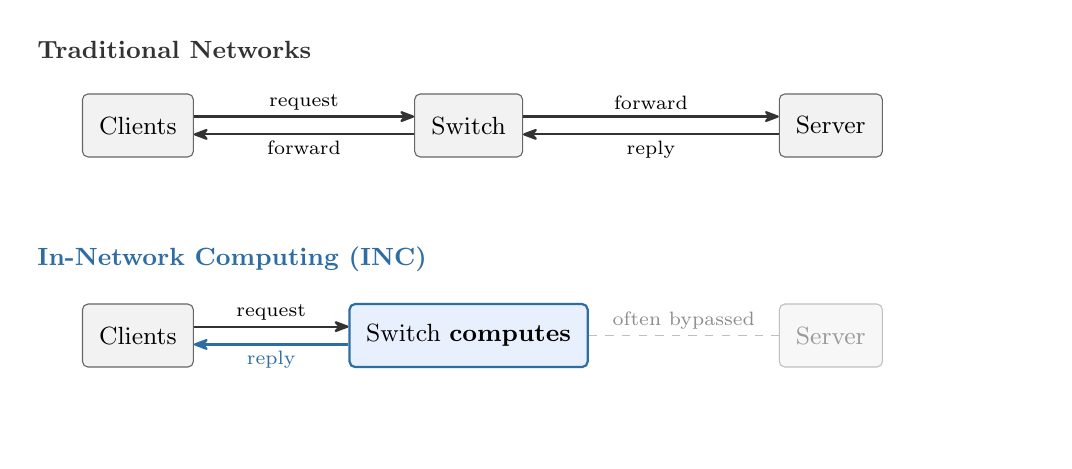
\begin{tikzpicture}[
    yscale=0.92,  % 压行距不压字号：节点文字不受 scale 影响，只有坐标被压
    every node/.style={font=\small},
    box/.style={draw, rounded corners=2pt, minimum height=8mm, inner xsep=6pt},
    host/.style={box, draw=cTextLight, fill=black!5},
    sw/.style={box, draw=cTextLight, fill=black!5},
    % 蓝而不是红：红色在这份 deck 里是 \alert 的颜色，第 3 帧拿它标丢包和违例。
    % 第 1 帧讲的是 INC 的好处，用红色会把"这里出问题了"的语义稀释掉。
    swhot/.style={box, draw=cHeader, thick, fill=cAccentLight},
    dim/.style={box, draw=black!25, fill=black!3, text=black!40},
    ar/.style={-{Stealth[round]}, thick, draw=cText},
    arhot/.style={-{Stealth[round]}, thick, draw=cHeader},
    lbl/.style={font=\scriptsize, inner sep=2pt},
    tag/.style={font=\small\bfseries, anchor=west},
  ]
  \useasboundingbox (-0.3,-1.25) rectangle (12.6,4.45);

  % ---------- 上：传统网络 ----------
  % 回程不绕路。原来那版从 Server 底下拉一条线绕回 Client，看着像把交换机
  % 跳过去了——而这张图恰恰要说交换机在两个方向上都只是转发。
  % 现在每一跳都是一条独立箭头：上行两段、下行两段，交换机两次 forward。
  \node[tag, text=cText] at (-0.3,4.15) {Traditional Networks};
  \node[host] (c1) at (1.1,3.1) {Clients};
  \node[sw]   (s1) at (5.3,3.1) {Switch};
  \node[host] (v1) at (9.9,3.1) {Server};

  \draw[ar] ([yshift=3.5pt]c1.east) -- node[lbl, above]{request}  ([yshift=3.5pt]s1.west);
  \draw[ar] ([yshift=3.5pt]s1.east) -- node[lbl, above]{forward}  ([yshift=3.5pt]v1.west);
  \draw[ar] ([yshift=-3.5pt]v1.west) -- node[lbl, below]{reply}   ([yshift=-3.5pt]s1.east);
  \draw[ar] ([yshift=-3.5pt]s1.west) -- node[lbl, below]{forward} ([yshift=-3.5pt]c1.east);

  \only<2->{
    % ---------- 下：INC ----------
    \node[tag, text=cHeader] at (-0.3,1.25) {In-Network Computing (INC)};
    \node[host]  (c2) at (1.1,0.2) {Clients};
    \node[swhot] (s2) at (5.3,0.2) {Switch \textbf{computes}};
    \node[dim]   (v2) at (9.9,0.2) {Server};

    \draw[ar]    ([yshift=3.5pt]c2.east) -- node[lbl, above]{request} ([yshift=3.5pt]s2.west);
    \draw[arhot] ([yshift=-3.5pt]s2.west) -- node[lbl, below, text=cHeader]{reply}  ([yshift=-3.5pt]c2.east);
    \draw[draw=black!25, dashed] (s2) -- node[lbl, above, text=black!45]{often bypassed} (v2);
  }
\end{tikzpicture}}

% 三个应用例子。不用 TikZ 手工定位——盒子宽度由文字决定，手给 x 坐标
% 必然有一天撞在一起（第一版就撞了，三个标签全被切掉右半）。
% 也不用 colorbox：三个色块加内边距就超出文本宽度，第三个会掉到第二行。
% 一行纯文字，\footnotesize（10pt，等效 21pt）——这是辅助信息，比正文小一档没问题。
\newcommand{\incexamples}{%
  {\centering\footnotesize
    Tensor aggregation {(SwitchML)}\ \textcolor{cHeader}{\textperiodcentered}\ 
    Key-value cache {(NetCache)}\ \textcolor{cHeader}{\textperiodcentered}\ 
    Lock manager {(NetLock)}\par}}
     % 第 1 帧的 INC 概念图（TikZ，随 overlay 分步出现）
% !TEX root = ../main.tex
% ============================================================
% 第 3 页：NetCache 的一致性违例 trace（重绘）
%
% 论文原图 1836x2468 竖长，16:9 页面上最宽只到 152pt，图内 45pt 的标签
% 缩到 3.7pt，投影上糊成一片。这里按投影重画，13cm 宽 1:1 排版不缩放。
%
% 排版上踩过的三个坑，改这张图前先读：
%
% 1. 消息名不要用数学模式。$W(V_1)$ 在 beamer 下排成 Computer Modern 的
%    数学斜体衬线体，而正文是 LMSans——一张图里两套字，看着就是乱。
%    统一用文本模式 + \textsubscript，字体自动跟正文走。
% 2. fill=white 只给真正压在泳道线上的标签。箭头标签用的是 above，本来就
%    在线的上方不压线，全都加白底的结果是满图白方块。
% 3. 不用 \emph。斜体在这张图里没有语义，只会再添一种字形。
%    要强调就用颜色和粗细——蓝=交换机自己的状态，红=出问题的地方。
%
% 丢掉的包画到半路就断、末端打叉：画到交换机上看着就像送到了。
% 每行至少空 0.3，否则会被上一行的箭头穿过。
% yscale 只压坐标不压字号。\useasboundingbox 固定画布，免得每个 overlay 图高不同。
% ============================================================
\newcommand{\msg}[1]{{\scriptsize #1}}          % 消息名：正体，跟正文同一套字
\newcommand{\vone}{V\textsubscript{1}}
\newcommand{\vtwo}{V\textsubscript{2}}

\newcommand{\netcachetrace}{%
\begin{tikzpicture}[
    yscale=0.80,
    every node/.style={font=\scriptsize},
    lane/.style={draw=black!30},
    lifeok/.style={draw=cHeader, line width=1.1pt},
    lifebad/.style={draw=black!38, line width=1.1pt, dash pattern=on 2pt off 2pt},
    head/.style={draw=cTextLight, rounded corners=2pt, fill=black!5,
                 minimum height=6.5mm, inner xsep=7pt, font=\small\bfseries},
    ar/.style={-{Stealth[round]}, draw=cText},
    arbad/.style={-{Stealth[round]}, draw=cRed, dashed},
    arhot/.style={-{Stealth[round]}, draw=cRed, thick},
    lbl/.style={inner sep=2pt},                        % 不加白底
    lblx/.style={inner sep=2pt},
    st/.style={inner sep=2pt, text=cHeader, font=\scriptsize\bfseries, anchor=east},
    stbad2/.style={inner sep=2pt, text=black!55, font=\scriptsize\bfseries, anchor=east},
    stbad/.style={inner sep=2pt, text=cRed, font=\footnotesize\bfseries},
    xmark/.style={font=\normalsize\bfseries, text=cRed, inner sep=0pt},
  ]
  \useasboundingbox (-0.35,-0.45) rectangle (12.95,6.05);

  \def\cx{1.15} \def\sx{6.3} \def\vx{11.5}

  \node[head] at (\cx,5.68) {Client};
  \node[head] at (\sx,5.68) {Switch};
  \node[head] at (\vx,5.68) {Server};
  % Switch 的生命线分段上色，用线本身表示缓存状态：蓝实线=有效，灰虚线=无效。
  % 这样状态不再占一行的高度（原来 "cache: invalid" 和 "cache: V1, valid"
  % 各吃掉一个行位，九步消息就排不开了），切换点只留一个很短的标签。
  % Client 和 Server 的生命线保持细灰线——这张图要看的是交换机怎么想。
  \only<2->{ \draw[lifeok] (\sx,5.35) -- (\sx,4.95); }
  \only<2>{  \draw[lifebad] (\sx,4.95) -- (\sx,-0.25); }
  \only<3->{
    \draw[lifebad] (\sx,4.95) -- (\sx,2.43);
    \draw[lifeok]  (\sx,2.43) -- (\sx,-0.25);
  }
  \only<2->{
    \draw[lane] (\cx,5.35) -- (\cx,-0.25);
    \draw[lane] (\vx,5.35) -- (\vx,-0.25);
  }

  % 第一个 overlay 不能是三条空泳道——那是两秒的空白。这两秒用来说明 NetCache
  % 本身怎么工作，trace 一开始跑就撤掉，把地方让给箭头。生命线从说明下方起，
  % 这样文字不压线，也不必给它铺白底。
  \only<1>{
    \foreach \x in {\cx,\sx,\vx} { \draw[lane] (\x,3.70) -- (\x,-0.25); }
    \node[text width=2.9cm, align=center, font=\footnotesize] at (\cx,4.55)
         {writes, then\\reads back};
    \node[text width=3.4cm, align=center, font=\footnotesize] at (\sx,4.55)
         {caches the item,\\answers reads itself};
    \node[text width=2.9cm, align=center, font=\footnotesize] at (\vx,4.55)
         {source of truth,\\keeps it in sync};
  }

  % 九行消息，行距统一 0.63。原来漏了服务器对 W(V2) 的回复——没有它，
  % 最后那个读就是和写并发的，而违例的前提恰恰是"读不与任何写并发"。
  % ---- overlay 2：写 V1，更新包丢了，客户端却收到了成功回复 ----
  \only<2->{
    \draw[ar] (\cx,4.95) -- node[lbl,above]{\msg{W(\vone)}} (\sx,4.95);
    \draw[ar] (\sx,4.95) -- node[lbl,above]{\msg{W(\vone)}} (\vx,4.95);
    \node[stbad2] at (\sx-0.06,4.55) {invalid};

    \draw[arbad] (\vx,4.32) -- node[lbl,above]{\msg{Upd(\vone)}} (\sx+1.45,4.32);
    \node[xmark] at (\sx+1.15,4.32) {$\times$};

    \draw[ar] (\vx,3.69) -- node[lbl,above,pos=0.72]{\msg{Reply[W(\vone)]}} (\cx,3.69);
  }

  % ---- overlay 3：写 V2 被挡住，重传的旧更新把缓存置成了 valid ----
  \only<3->{
    \draw[ar] (\cx,3.06) -- node[lbl,above]{\msg{W(\vtwo)}} (\sx,3.06);
    \draw[ar] (\sx,3.06) -- node[lbl,above]{\msg{W(\vtwo)}} (\vx,3.06);
    \node[anchor=west, font=\scriptsize\bfseries, inner sep=2pt]
         at (\vx+0.12,2.79) {blocked};

    \draw[ar] (\vx,2.43) -- node[lbl,above]{\msg{Upd(\vone)} retransmitted} (\sx,2.43);
    \node[st] at (\sx-0.06,2.03) {valid: \vone};
  }

  % ---- overlay 4：新的更新又丢了，读命中一个自以为有效的缓存 ----
  % 读和回复分两行，不合成双向箭头：中间隔着交换机的一次判断——它认为自己
  % 的缓存有效，才从缓存里答的。画成一条往返就把那个判断藏掉了。
  \only<4->{
    \draw[arbad] (\vx,1.80) -- node[lbl,above]{\msg{Upd(\vtwo)}} (\sx+1.45,1.80);
    \node[xmark] at (\sx+1.15,1.80) {$\times$};

    \draw[ar] (\vx,1.17) -- node[lbl,above,pos=0.72]{\msg{Reply[W(\vtwo)]}} (\cx,1.17);

    \draw[ar] (\cx,0.54) -- node[lbl,above]{\msg{R}} (\sx,0.54);
    \draw[arhot] (\sx,-0.09) -- node[lbl,above,text=cRed]{\msg{\vone\ --- stale}} (\cx,-0.09);
  }
\end{tikzpicture}}
  % 第 3 帧的违例 trace（TikZ 重绘，论文原图投影上糊掉）

\input{speech-notes}   % 由 speech2tex.py 从 speech.md 生成

\begin{document}

\darktitlepage[1]   % 可选参数 = 封面讲稿段号（speech.md 的 **P1.**）

% \section{} 仍然写着，因为 frametitle 上的进度条要靠它；只是 sectionpage=none
% （见 preamble），章节不单独出页。
% !TEX root = ../main.tex
\section{The Problem}

\begin{frame}{Computation Is Moving Into the Switch}
  \vspace{0.2em}
  \begin{center}\incconcept\end{center}
  \vspace{0.1em}
  % \visible 而不是 \only：\only 不占位，这行例子一出现会把上面整块往上推 11pt
  \visible<3->{\incexamples}
  \speechnote{2}
\end{frame}

\begin{frame}{Why Correctness Is Hard Here}
  \vspace{0.6em}
  \begin{itemize}
    \item[] \textbf{Network unreliability leads to computational errors.}\\
            TCP makes delivery reliable \emph{between the endpoints}.
            The switch in the middle still sees loss, duplication and reordering.
    \vspace{1.0em}
    \item[]<2-> \textbf{And the switch cannot recover from them.}\\
            No loops. One memory access per pipeline stage.
            No reliable transport in the data plane.
  \end{itemize}
  \vspace{1.2em}
  \visible<3->{%
    \begin{center}
      \begin{minipage}{0.92\textwidth}
        \centering
        \alert{This is what distinguishes INC from a traditional distributed system:}\par
        \alert{there, every node is a general-purpose server}\par
        \alert{with rich computation and storage resources.}
      \end{minipage}
    \end{center}}
  \speechnote{3}
\end{frame}

\begin{frame}{NetCache Returns a Value That Was Overwritten}
  \vspace{0.1em}
  \begin{center}\netcachetrace\end{center}
  \vspace{0.2em}
  \begin{center}
    \begin{minipage}{0.94\textwidth}
      \centering
      \only<1>{{A write-through cache. Watch what the switch believes about it.}}%
      \only<2>{The client is told the write succeeded --- but the cache never heard about it.}%
      \only<3>{The retransmitted \emph{old} update marks the cache valid again.}%
      \only<4>{\alert{\textbf{Cache consistency is violated: the read is not concurrent with any write, but does not get the latest value.}}}%
    \end{minipage}
  \end{center}
  \speechnote{4}
\end{frame}

\begin{frame}{This Is Not Something You Find by Thinking Harder}
  \vspace{0.4em}
  Two specific losses, in one specific interleaving.
  \vspace{0.5em}

  Protocols get designed for a reliable network,
  then \emph{patched} for the exceptions. That fails three ways.
  \vspace{0.9em}
  \begin{itemize}
    \item The exceptions you never thought of are never patched
    \item A patch addresses one specific exception, not the root cause
    \item Patches conflict with each other once several exceptions co-occur
  \end{itemize}
  \vspace{1.0em}
  \begin{center}
    \alert{Synthetic workloads and simulators do not exhaustively enumerate these.}
  \end{center}
  \speechnote{5}
\end{frame}

\begin{frame}{Existing Verification Does Not Answer This}
  \vspace{0.8em}
  \begin{itemize}
    \item \textbf{Network verification} checks routing ---
          reachability, loops, isolation.\\
          {No computation involved.}
    \vspace{0.8em}
    \item \textbf{HSA and NetSMC} assume a stateless network,
          or reason about one packet at a time.\\
          INC switches hold state across many related packets.
    \vspace{0.8em}
    \item \textbf{P4 program verifiers} (p4v, Vera, Aquila)
          check the \emph{implementation}.\\
          We ask whether the \emph{design} itself is correct.
  \end{itemize}
  \speechnote{6}
\end{frame}

% !TEX root = ../main.tex
\section{VeriNC}

\begin{frame}{VeriNC}
  \begin{center}
    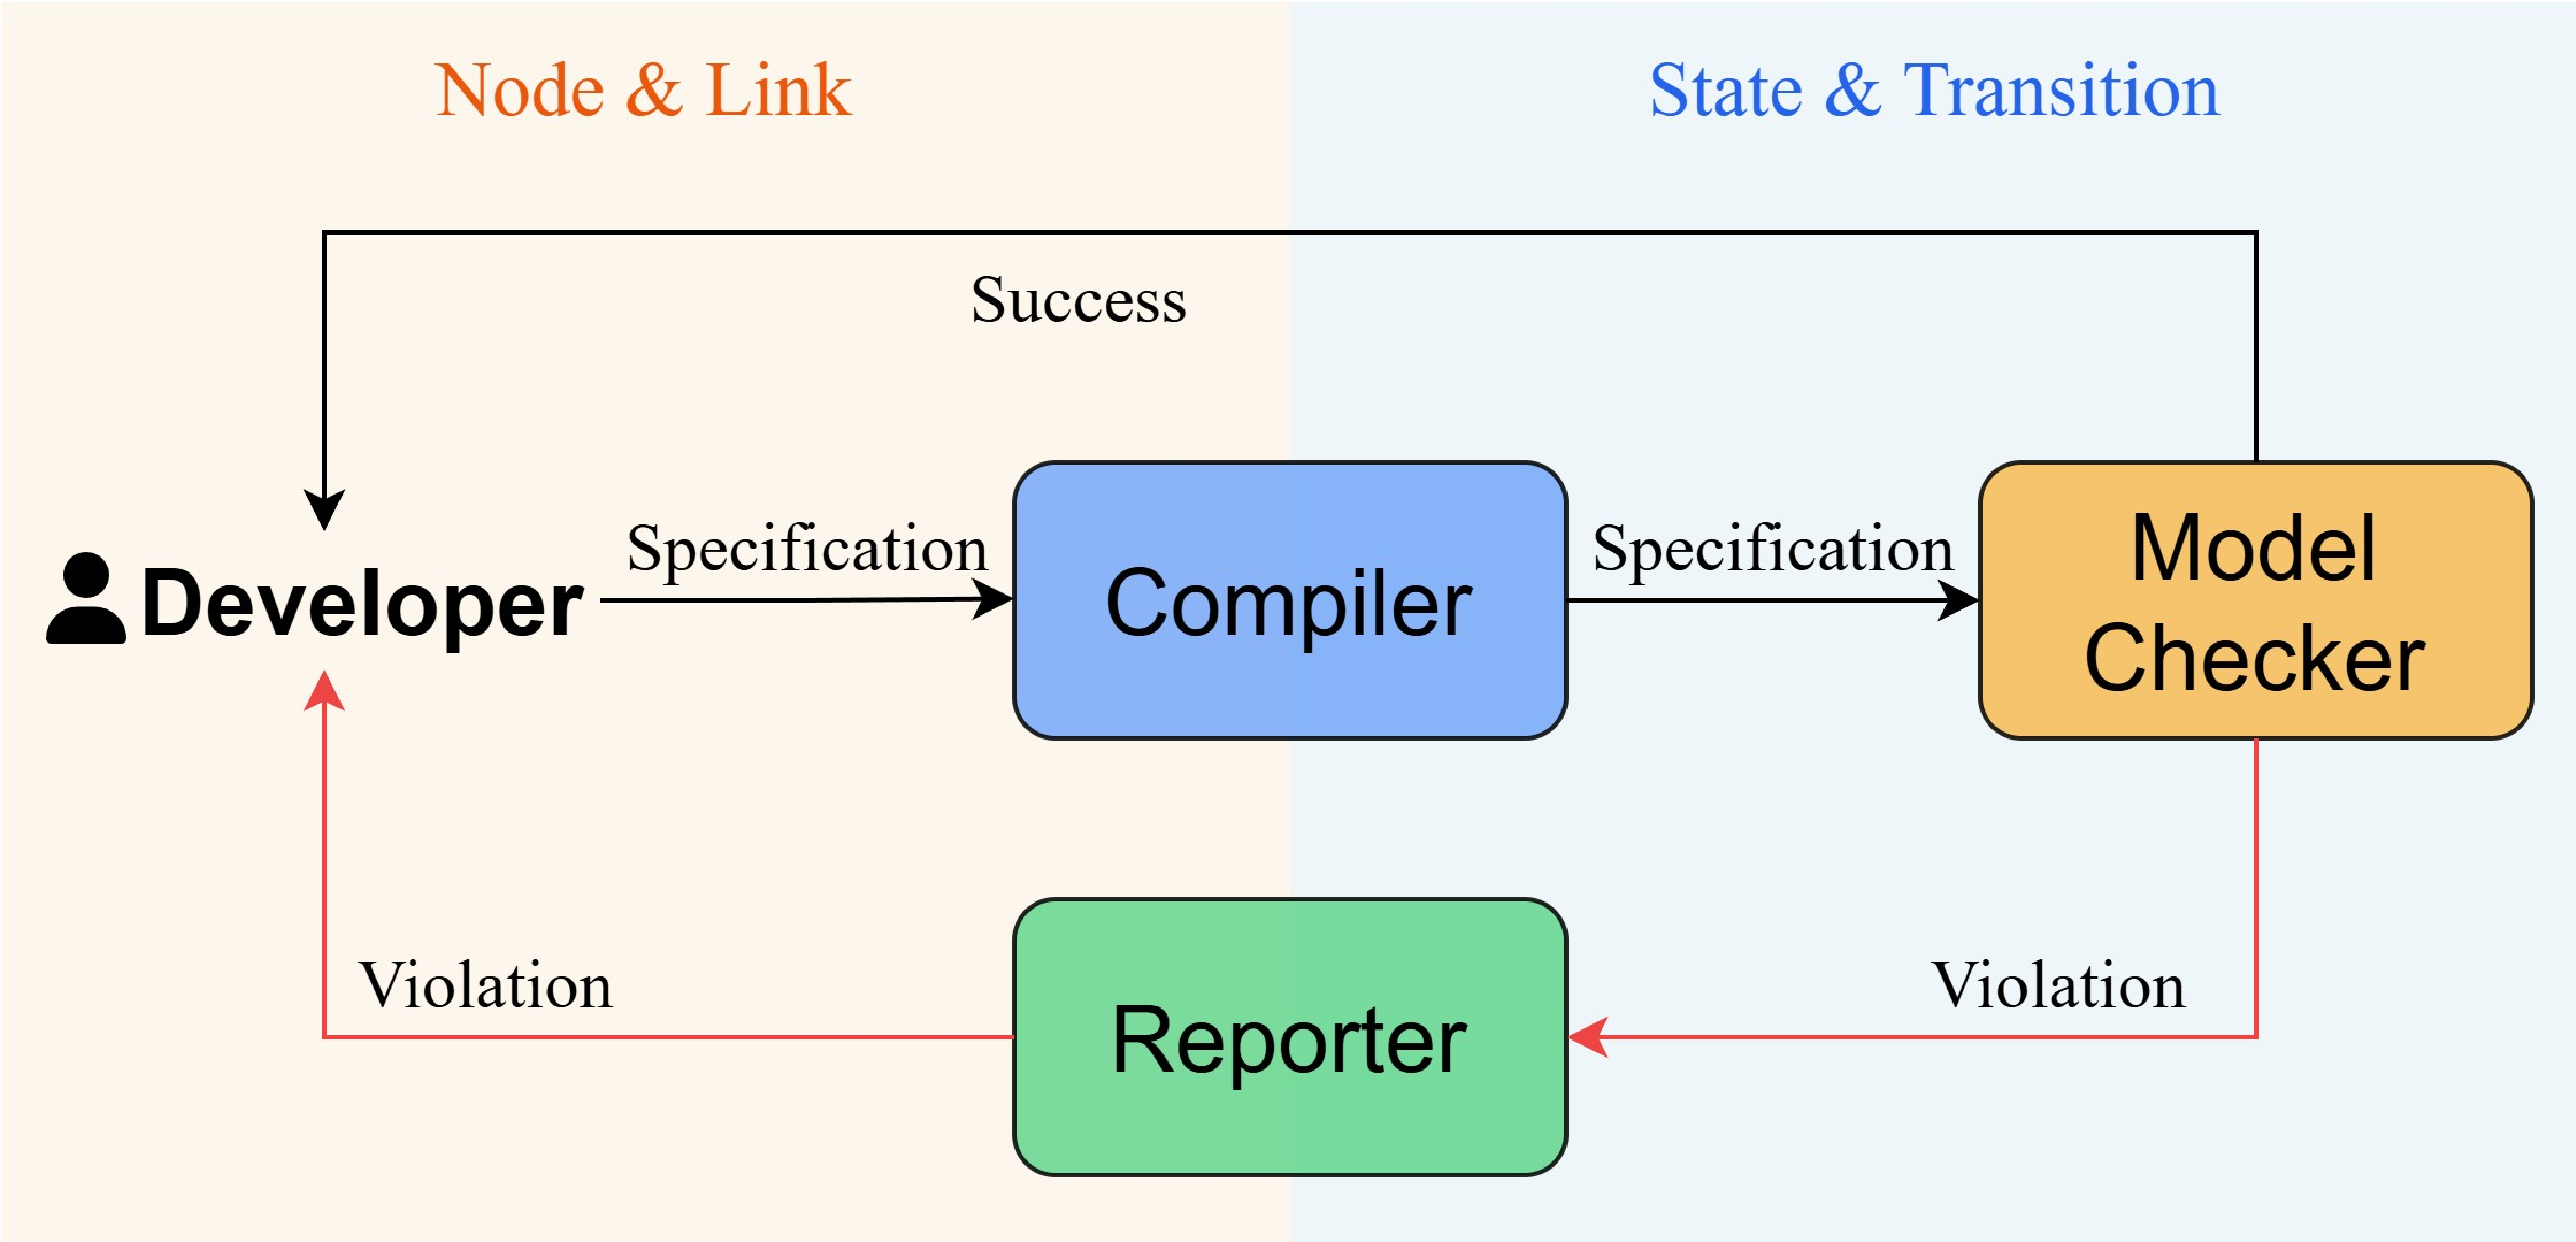
\includegraphics[width=0.70\textwidth]{figures/workflow.pdf}
  \end{center}
  \vspace{0.7em}
  \begin{center}
    \begin{minipage}{0.90\textwidth}
      \centering
      \alert{\textbf{VeriNC explores all possible execution traces ---
      exhaustively, within the bounds you set.}}
    \end{minipage}
  \end{center}
  \speechnote{7}
\end{frame}

\begin{frame}{The Abstraction You Work In}
  \vspace{0.5em}
  \begin{itemize}
    \item A \textbf{node} is a machine, running several \textbf{threads} ---
          application, receive, retransmission.\\
          {Threads run concurrently; every interleaving gets explored.}
    \vspace{0.7em}
    \item<2-> Nodes are joined by \textbf{links}. Three primitives:
          \texttt{Send}, \texttt{Receive}, \texttt{Multicast}.
    \vspace{0.7em}
    \item<3-> The network is \textbf{reliable}, \textbf{lossy}, or \textbf{out-of-order} ---
          set globally, or per link.
  \end{itemize}
  \vspace{1.0em}
  \visible<4->{%
    \begin{center}
      \begin{minipage}{0.92\textwidth}
        \centering
        % 手动断行：自己折的话 "itself." 会单独掉到第二行
        \alert{\textbf{Users specify protocol behavior\\
        without modeling the network itself.}}
      \end{minipage}
    \end{center}}
  \speechnote{8}
\end{frame}

\begin{frame}[fragile]{What You Actually Write}
  \vspace{0.2em}
  \begin{center}
    \begin{minipage}{0.88\textwidth}
\begin{lstlisting}[style=spec, basicstyle=\ttfamily\footnotesize]
configuration {
  MAX_LOSS = 1;  CLIENT_NUM = 3;  REQ_NUM = 5;  ...
}
topology {
  nodetype Client, Switch, Controller, Server;
  link c1, c2, c3 -- sw -- ctrl, s;  ...
}
protocol {
  var(Switch) cached = 0, valid = 0, value = null;  ...
  thread(Switch) SwitchRecv { ... }
}
\end{lstlisting}
    \end{minipage}
  \end{center}
  \vspace{0.4em}
  \begin{center}
    \alert{Protocol logic, not P4 --- the core logic, without implementation detail.}
  \end{center}
  \speechnote{9}
\end{frame}

\begin{frame}[fragile]{Saying What Correctness Means}
  \vspace{1.2em}
  \begin{itemize}
    \item An \textbf{assert statement} --- a first-order logic formula,
          checked where it sits
    \vspace{1.0em}
    \item A \textbf{property} block in LTL, checked after every transition\\[0.4em]
          \hspace*{1.2em}\texttt{[]} always \qquad \texttt{<>} eventually
    \vspace{1.0em}
    \item A \textbf{stateful check function}, for complex temporal properties
  \end{itemize}
    \speechnote{10}
\end{frame}

% !TEX root = ../main.tex
\section{Making It Tractable}

\begin{frame}{Challenge: The State Space Explodes}
  \vspace{0.4em}
  Every packet may be dropped, reordered, or retransmitted at any moment.
  \vspace{1.0em}
  \begin{itemize}
    \item<2-> \textbf{INC objects are usually logically independent.}\\
          So we model just one of them.
    \vspace{0.6em}
    \item<3-> \textbf{Nodes of the same type are symmetric.}\\
          So we explore one arrangement and discard its permutations ---
          without losing completeness.
    \vspace{0.6em}
    \item<4-> \textbf{A little unreliability is usually enough.}\\
          So we constrain it: a maximum number of losses, reorderings
          and duplicates.
  \end{itemize}
  \speechnote{11}
\end{frame}

\begin{frame}{What It Costs to Run}
  \vspace{0.2em}
  \begin{center}
    \footnotesize
    \renewcommand{\arraystretch}{0.95}
    \begin{tabular}{@{}lrrr@{}}
      \toprule
      \textbf{System} & \textbf{VeriNC} & \textbf{TLA\textsuperscript{+}}
        & \textbf{To first violation} \\
      \midrule
      FissLock  & 466 & 1053 & 1\,s \\
      SwitchML  &  98 &  440 & 3\,s \\
      NetCache  & 190 &  589 & 8\,s \\
      NetReduce & 146 &  486 & 72\,s \\
      \bottomrule
    \end{tabular}
  \end{center}
  \vspace{0.6em}
  \begin{center}
    \begin{minipage}{0.94\textwidth}
      \centering
      % 手动断行：自己折的话 "to." 会单独掉到第二行
      On average the specification is \textbf{67.2\% shorter}\\
      than the TLA\textsuperscript{+} it compiles to.
      \vspace{0.5em}

      Violations usually sit in the \emph{shallow} layers of the state space,
      so breadth-first search reaches them early.
    \end{minipage}
  \end{center}
  \speechnote{12}
\end{frame}

% !TEX root = ../main.tex
\section{What We Found}

\begin{frame}{Seven of Nine Systems Violate Properties}
  \begin{center}
    \footnotesize
    \renewcommand{\arraystretch}{0.95}
    \begin{tabular}{@{}llc@{}}
      \toprule
      \textbf{System} & \textbf{Property violated} & \textbf{Network} \\
      \midrule
      SwitchML  & computational correctness & out-of-order \\
      ATP       & memory leak freedom       & out-of-order \\
      NetReduce & terminality               & lossy \\
      \addlinespace[0.45em]
      NetCache  & cache consistency & lossy \\
      NetCache  & terminality       & reliable \\
      FarReach  & cache consistency & reliable \\
      \addlinespace[0.45em]
      NetLock   & lock exclusion & delayed \\
      FissLock  & lock exclusion & delayed \\
      \bottomrule
    \end{tabular}
  \end{center}
  \vspace{0.7em}
  \begin{center}
    \begin{minipage}{0.94\textwidth}
      \centering
      \visible<2->{Few of these systems explicitly state their network assumptions.}
    \end{minipage}
  \end{center}
  \speechnote{13}
\end{frame}

\begin{frame}{Not Just on Paper}
  \vspace{0.5em}
  \begin{itemize}
    \item Following each violation trace, we injected exactly those losses
          and delays into the \textbf{real open-source implementations}.
    \vspace{0.7em}
    \item<2-> \textbf{All six open-source systems reproduced the violation.}
    \vspace{0.7em}
    \item<3-> The authors of \textbf{ATP} and \textbf{NetReduce} confirmed these
          were oversights at design time.
    \vspace{0.7em}
    \item<4-> \textbf{EPIC} (SIGCOMM~'26) used VeriNC \emph{during} its design ---
          a buffer management pitfall was fixed before publication.
  \end{itemize}
  \speechnote{14}
\end{frame}

\begin{frame}{Three Patterns Behind Those Violations}
  \vspace{0.6em}
  \begin{itemize}
    \item \textbf{Stale packets pollute switch state.}\\
          {Give the switch a way to recognize them.}
    \vspace{0.8em}
    \item \textbf{Concurrent events race with no coordination.}\\
          {Handle how events interact, not one event at a time.}
    \vspace{0.8em}
    \item \textbf{Unreliability turns a latent risk into a real violation.}\\
          {Most of what we found needs only a single such event.}
  \end{itemize}
  \speechnote{15}
\end{frame}

\begin{frame}{Conclusion}
  \vspace{0.6em}
  % 条目间距用 itemsep 统一给，不要逐条插 \vspace——手插的间距在折行的条目
  % 之间表现不一致，三条看着一条比一条挤。preamble 的钩子把 itemsep 设成 2pt，
  % 在环境内部再设一次就能盖掉（钩子先执行）。
  \begin{itemize}
    \setlength{\itemsep}{0.9em}
    \item \textbf{Design-level verification} for in-network computing systems
    \item A high-level \textbf{specification language} and
          \textbf{configurable network environments}
    \item Nine systems modeled; design risks in seven of them, found in
          seconds and reproduced on the real implementations
  \end{itemize}
  \vspace{1.0em}
  \begin{center}
    \begin{minipage}{0.94\textwidth}
      \centering
      \alert{\textbf{Formal modeling and verification are an essential step}}\par
      \alert{\textbf{in driving the deployment of INC systems.}}
    \end{minipage}
  \end{center}
  \speechnote{16}
\end{frame}


% ============ 结束页 ============
% standout 帧的两个坑：紧跟 {...} 会被当 frametitle 吃掉（先放 \vspace*{0pt}）；
% 帧内不能用 \\（dual 模式报 There's no line here to end）。
\begin{frame}[standout]
  \vspace*{0pt}

  {\Large Thank you}

  \vspace{1.0em}
  {\large Questions?}

  \vspace{1.4em}
  {\footnotesize\texttt{github.com/cs-icez/verinc-compiler}}

  {\footnotesize\texttt{github.com/cs-icez/verinc-violation}}

  \vspace{0.8em}
  {\footnotesize tianyubai@stu.pku.edu.cn}
\end{frame}

\end{document}
